\documentclass[a4paper,12pt]{article}
%\documentclass[a4paper,10pt]{scrartcl}

\usepackage[utf8x]{inputenc}
\usepackage{amsfonts}
\usepackage{amsmath,esint}
\usepackage{graphicx}
\usepackage{pdfpages}
\usepackage{sansmath}
\usepackage{hyperref}
\usepackage{natbib}
\usepackage{caption}
\usepackage{subcaption}

\usepackage{tikz}


\definecolor{boiseBlue} {RGB}{29,72,159}
\definecolor{rojoAmor} {RGB}{171,13,4}
\definecolor{moradoAmor} {RGB}{93,8,113}
\definecolor{verdeAmor} {RGB}{98,158,31}
\definecolor{negro} {RGB}{10,10,10}
\definecolor{lgreen} {RGB}{180,210,100}
\definecolor{dblue}  {RGB}{20,66,129}
\definecolor{ddblue} {RGB}{11,36,69}
\definecolor{lred}   {RGB}{220,0,0}
\definecolor{nred}   {RGB}{224,0,0}
\definecolor{norange}{RGB}{230,120,20}
\definecolor{nyellow}{RGB}{255,221,0}
\definecolor{ngreen} {RGB}{98,158,31}
\definecolor{dgreen} {RGB}{78,138,21}
\definecolor{nblue}  {RGB}{28,130,185}
\definecolor{jblue}  {RGB}{20,50,100}

\usepackage{listings}
\usepackage{xcolor}
\usepackage{verbatim}
\lstset{language=C++,
	basicstyle=\ttfamily,
	backgroundcolor=\color{black!5}\ttfamily,
	keywordstyle=\color{nblue}\ttfamily,
	stringstyle=\color{nred}\ttfamily,
	commentstyle=\color{ngreen}\ttfamily,
	morecomment=[l][\color{moradoAmor}]{\#}
}

\newenvironment{rcases}{\left.\begin{aligned}}{\end{aligned}\right\rbrace}

\renewcommand{\familydefault}{\sfdefault}

\newcommand{\specialcell}[2][c]{%
	\begin{tabular}[#1]{@{}c@{}}#2\end{tabular}}
% \specialcell{Foo\\bar}

\title{Two-dimensional diffusion\\{\normalsize Diego Domenzain, Fall 2022}}
\author{}
\date{}

\pdfinfo{%
	/Title    ()
	/Author   ()
	/Creator  ()
	/Producer ()
	/Subject  ()
	/Keywords ()
}

\begin{document}
	\maketitle
	\iffalse
	%-------------------
	% main flow
	%-------------------
	\section*{2D wave equation}
	Let $\nabla=(\partial_x,\partial_z)$ be a row vector.
	\begin{align}
		{\bf C}\dot{{\bf v}} &= \nabla u - {\bf A}{\bf v} + {\bf g}\\
		c\dot{u} &= \nabla\cdot{\bf v} - a u + f
	\end{align}
	Velocity is determined by ${\bf C}$ and $c$. Intrinsic attenuation is determined by ${\bf A}$ and $a$.
	\\\\
	%
	In expanded-matrix form we have,
	\begin{align}
		\begin{pmatrix} 
			c_{11} & c_{12} & 0\cr 
			c_{21} & c_{22} & 0 \cr
			0 & 0 & c
		\end{pmatrix}
		%
		\begin{pmatrix} 
			\dot{v}_x \cr
			\dot{v}_z \cr
			\dot{u}
		\end{pmatrix}
		%
		=
		%
		&
		\begin{pmatrix} 
			0 & 0 & \partial_x \cr 
			0 & 0 & \partial_z \cr
			\partial_x & \partial_z & 0
		\end{pmatrix}
		%
		\begin{pmatrix} 
			v_x \cr
			v_z \cr
			u
		\end{pmatrix}
		%
		%
		-\\
		%
		&
		\begin{pmatrix} 
			a_{11} & a_{12} & 0\cr 
			a_{21} & a_{22} & 0 \cr
			0 & 0 & a
		\end{pmatrix}
		%
		\begin{pmatrix} 
			v_x \cr
			v_z \cr
			u
		\end{pmatrix}
		%
		+
		%
		\begin{pmatrix} 
			g_x \cr
			g_z \cr
			f
		\end{pmatrix}.
	\end{align}
	Note that this equation can handle anisotropy and attenuation acting on {\bf v}.
	\clearpage
	\fi
	% ----------------------------
	% 2.5d wave
	% ----------------------------
	\section*{2D EM wave equation}
	\begin{align}
		\boldsymbol{\mu}\dot{{\bf H}} &= -\nabla\times{\bf E} + {\bf M}_s\\
		\boldsymbol{\varepsilon}\dot{{\bf E}} &= \nabla\times{\bf H} - \boldsymbol{\sigma}{\bf E} - {\bf J}_s
	\end{align}
	Assuming quasi-isotropic materials and $\partial_y=0$, in expanded-matrix form we have the TE mode,
	\begin{align}
		\begin{pmatrix} 
			\mu & 0 & 0\cr 
			0 & \mu & 0 \cr
			0 & 0 & \varepsilon
		\end{pmatrix}
		%
		\begin{pmatrix} 
			-\dot{H}_z \cr
			\dot{H}_x \cr
			\dot{E}_y
		\end{pmatrix}
		%
		=
		%
		&
		\begin{pmatrix} 
			0 & 0 & \partial_x \cr 
			0 & 0 & \partial_z \cr
			\partial_x & \partial_z & 0
		\end{pmatrix}
		%
		\begin{pmatrix} 
			-H_z \cr
			H_x \cr
			E_y
		\end{pmatrix}
		%
		%
		-\\
		%
		&\sigma
		\begin{pmatrix} 
			0 \cr
			0 \cr
			E_y
		\end{pmatrix}
		%
		+
		%
		\begin{pmatrix} 
			M_z \cr
			M_x \cr
			-J_y
		\end{pmatrix}.
	\end{align}
	The terms $M_z,\,M_x,$ and $J_y$ are the source terms for $H_z,\,H_x,$ and $E_y$ respectively. The velocity of propagation is given by $v=1/\sqrt{\mu\varepsilon}$.
	\\\\
	For example, when modeling an electric dipole antenna parallel to the $y$-axis, then $M_z=M_x=0$, and only $J_y$ varies as a function of time. When modeling a magnetic dipole antenna parallel to the $z$-axis, then $J_y=M_x=0$, and only $M_z$ varies as a function of time.
	\\\\
	An EM field exhibits wave propagation when the media is a {\it poor conductor},
	\begin{align}
		\frac{\sigma}{\omega\varepsilon} << 1,
	\end{align}
	where $\omega=2\pi f_o$ and $f_o$ is the fundamental frequency of the source term.
	% ----------------------------
	% 2.5d wave
	% ----------------------------
	\section*{2D EM diffusion}
	An EM field exhibits diffusion propagation when the media is a {\it good conductor},
	\begin{align}
		1 << \frac{\sigma}{\omega\varepsilon}.
	\end{align}
	We re-write the {\it good/bad conductor} conditions as follows,
	\begin{align}
		\varepsilon &>> \frac{\sigma}{\omega} &\text{ poor conductor},\\
		\varepsilon &<< \frac{\sigma}{\omega} &\text{ good conductor}.
	\end{align}
	Now, by looking at Greens solutions for wave and diffusion propagation it can be shown that they agree asymptotically when \cite[]{oristaglio1984diffusion},
	\begin{align}
		\frac{2\varepsilon}{\sigma} << \sqrt{t^2 - \frac{r^2}{v^2}},
	\end{align}
	where $r$ is the distance from source to receiver and $t$ is the time it takes for the field to arrive to the receiver.
	\\\\
	We can re-write this equation in order to get a criteria on when propagation is diffusive,
	\begin{align}
		r^* = \sqrt{v^2 \cdot \left(t^2 - \frac{4\varepsilon^2}{\sigma^2}\right)}.
	\end{align}
	The difference between $r$ and $r^*$ is that $r$ is the real distance between source and receiver, and $r^*$ is a function of $v,\,t,\,\varepsilon,$ and $\sigma$.
	% ----------------------------
	% 2.5d wave
	% ----------------------------
	\section*{Is it EM diffusion or wave propagation?}
	First, we can plot $\sigma/\omega$. If the target values for $\varepsilon$ are below those of the plot, then it is diffusion. See Figure \ref{fig:conductmedia}.
	\\\\
	Then, for a fixed value of $\varepsilon$ we can plot $r^*$ (Figure \ref{fig:wavevsdiffu}). Then we compare with our survey acquisition,
	\begin{itemize}
		\item if $r<<r^*$ it is diffusion,
		\item if $0<r^*<<r$ it is on the edge of being a wave or diffusion,
		\item if $r^*\in\mathbb{C}$ it is a wave.
	\end{itemize}
	% --
	\begin{figure}[h!]
		\centering
		\begin{subfigure}[b]{0.7\linewidth}
			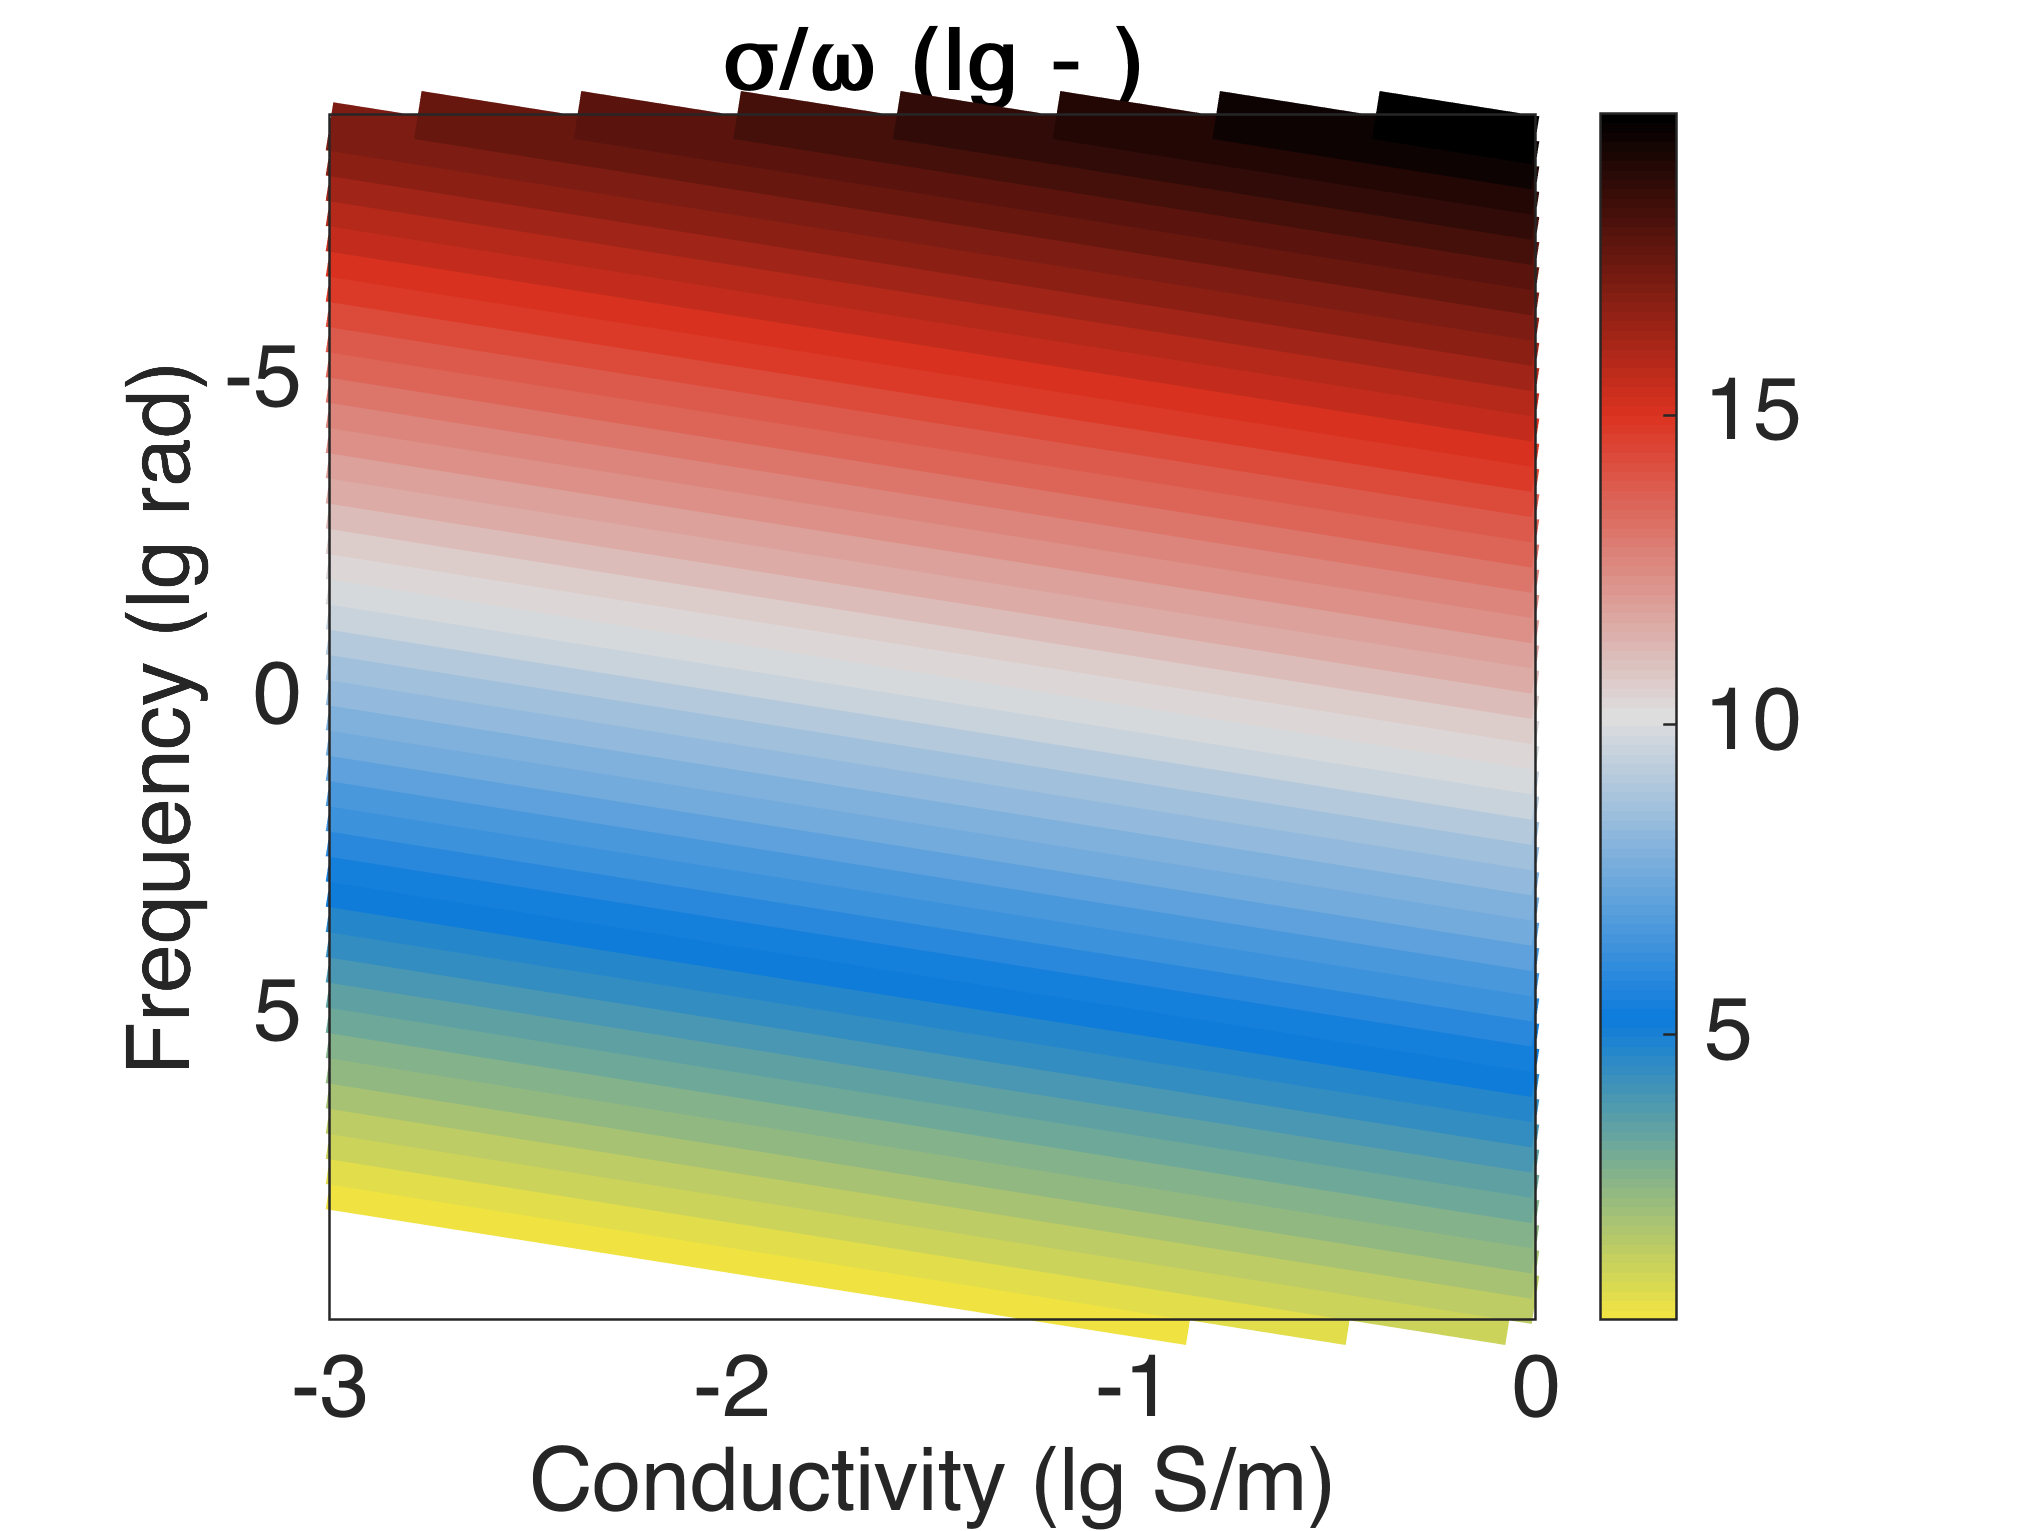
\includegraphics[width=\linewidth]{conductmedia.png}
			\caption{\centering For crazy large would-be values of relative permittivity (colors), the media is diffusive.}
			\label{fig:conductmedia}
		\end{subfigure}
		\begin{subfigure}[b]{0.7\linewidth}
			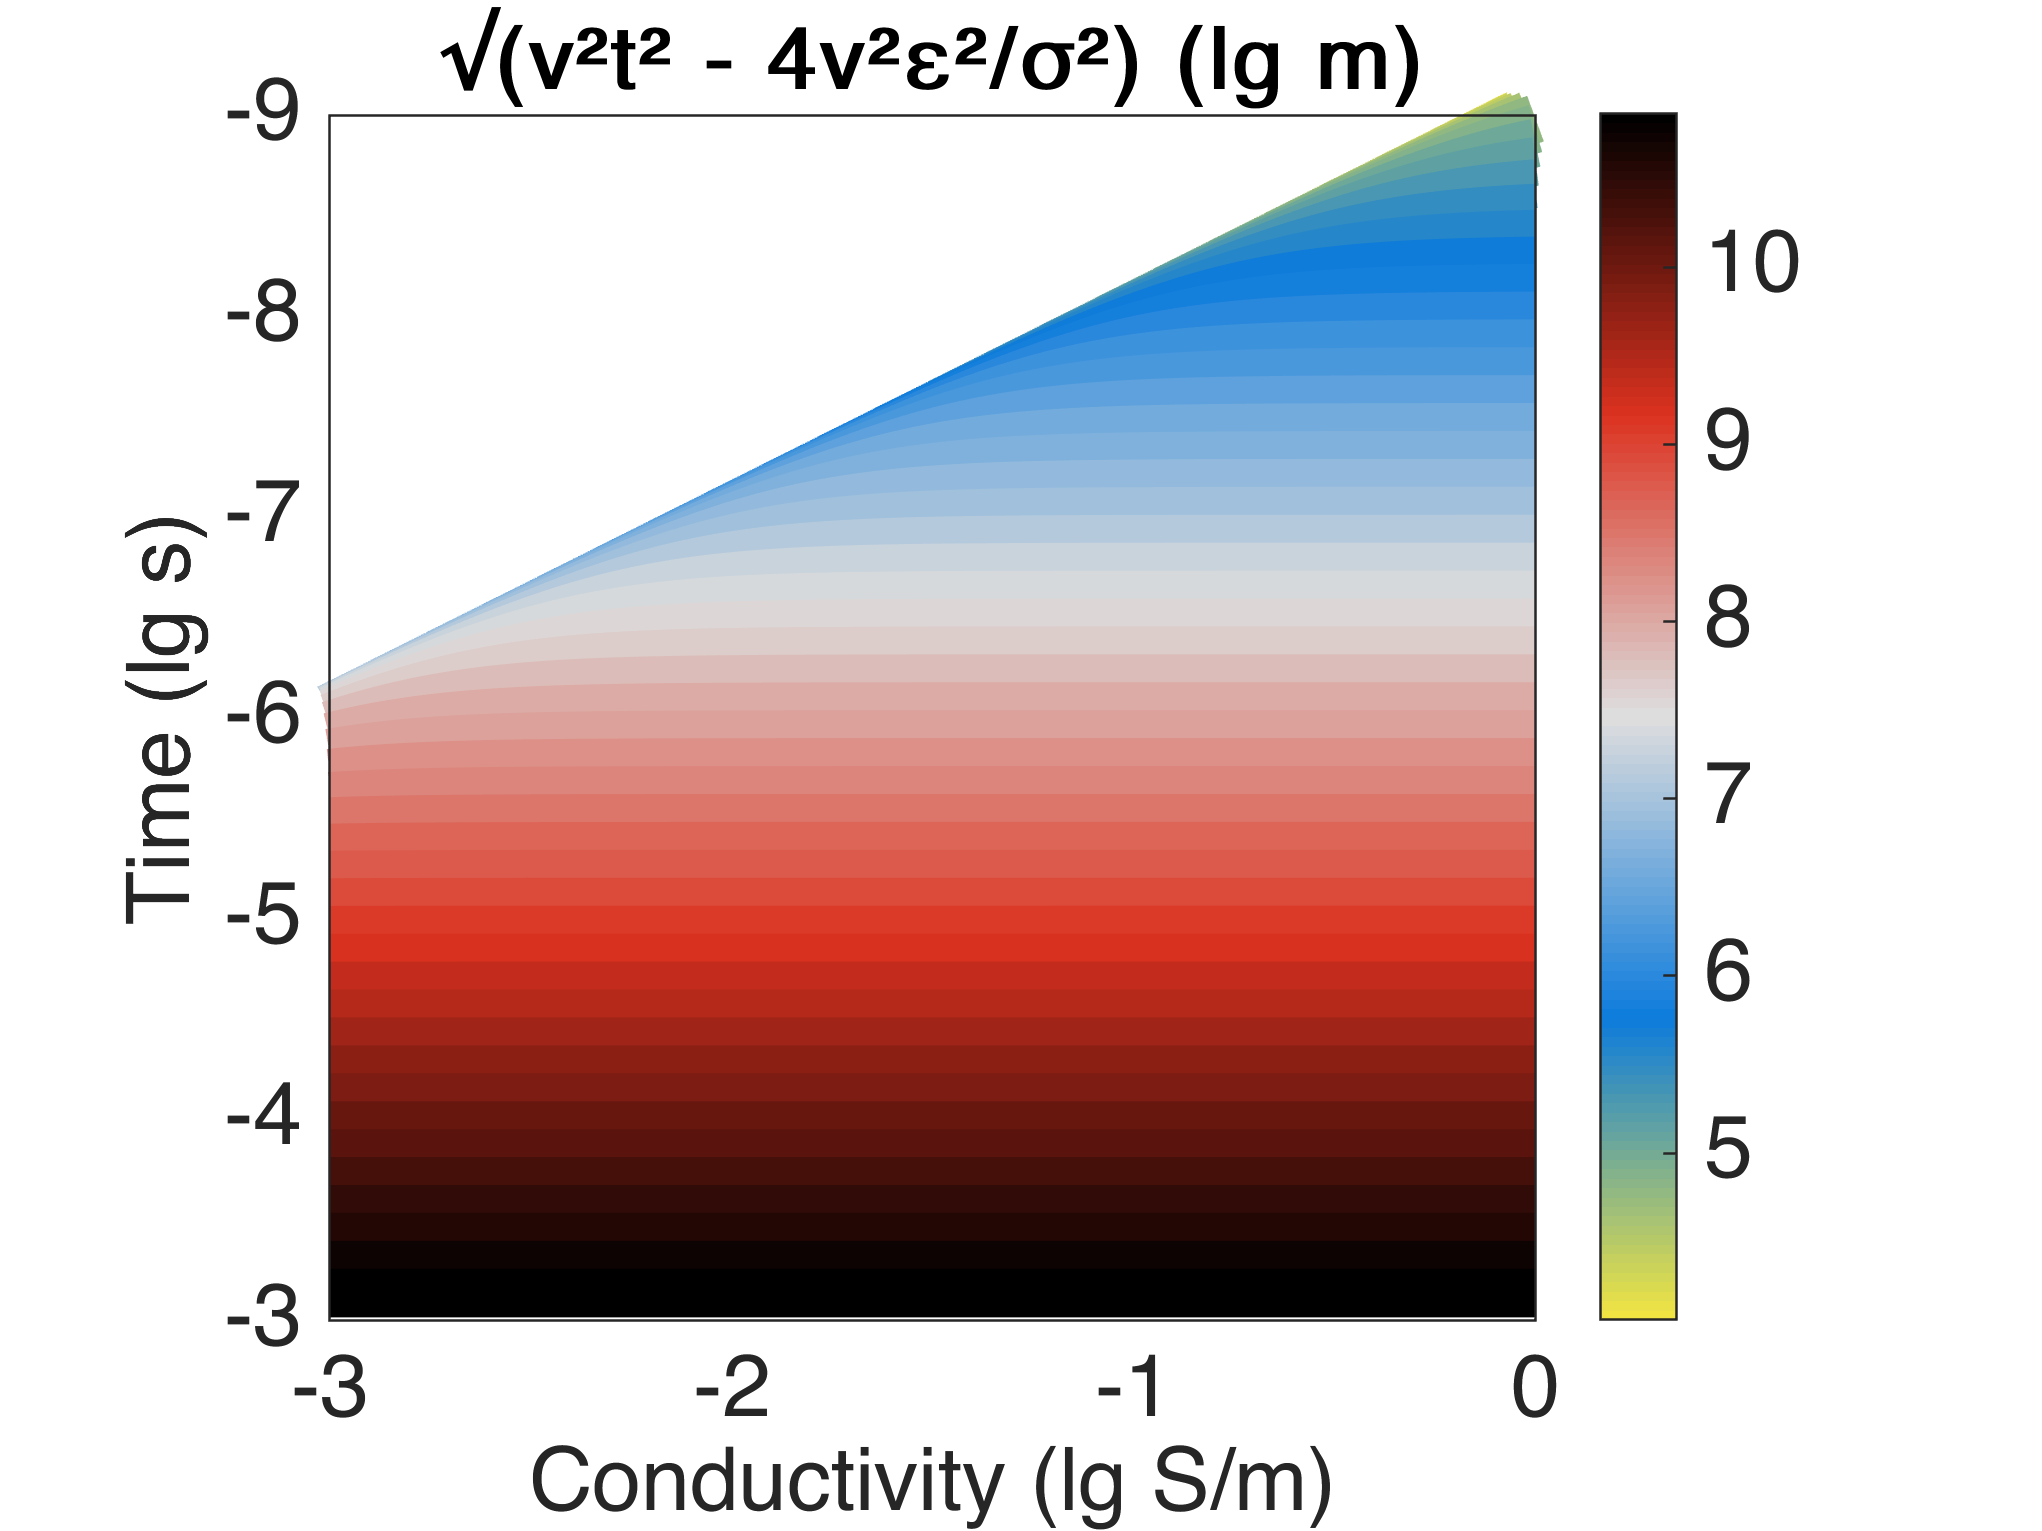
\includegraphics[width=\linewidth]{wavevsdiffu.png}
			\caption{\centering If your receiver is placed at distances much shorter than $r^*$ (colors) then there is no difference between wave and diffusion. In this case $\varepsilon_r = 50$ just because.}
			\label{fig:wavevsdiffu}
		\end{subfigure}
		\caption{{\bf Can I use my wave code to solve for diffusion?}}
	\end{figure}
	% ----------------------------
	% 2.5d wave
	% ----------------------------
	\section*{Comments on a magnetic dipole source}
	The EM system HGG uses is a magnetic source driven by a {\it square} wired coil. I think the modeling team got confused and modeled a square coil as two electric dipoles. That would explain the in-out motion of the electric field in the gif.
	\\\\
	If the coil is actually a coil and not two electric dipoles, then the induced source is a magnetic dipole and not two infinitely long electric dipoles. So the modeling team got that wrong.
	%
	%
	%------------
	% biblio
	%------------
	%\newpage
	\bibliographystyle{plainnat}
	\bibliography{2dtem}
	%\nocite{*}
\end{document}